\section*{Results}
The paired comparison evaluates eight input-permission conditions for three models, three split seeds and two hospitals. It produces 144 discrimination records and 288 fixed-policy records. Full-input scores are recomputed and checked against the saved parent predictions before any intervention. Every reference-versus-reference contrast has zero difference by construction; restricted comparisons use the same patients and thresholds rather than independently selected test samples.



Every non-reference permission condition reduces mean AUROC within each model--hospital combination, although the size of the change varies substantially. At hospital A, boosting changes from 0.794 with full inputs to 0.780, 0.763 and 0.747 at per-group denial probabilities of 0.1, 0.3 and 0.5. Its corresponding hospital-B values are 0.731, 0.716, 0.688 and 0.662. At probability 0.3, the mean AUROC decrease ranges from 0.019 to 0.051 across the six model--hospital combinations. These averages describe three overlapping patient splits; they are not independent-cohort meta-analytic estimates.

The source being restricted matters as much as the overall amount of available information. For the GRU at hospital B, removing all laboratories changes mean AUROC from 0.752 to 0.745, whereas removing all vitals reduces it to 0.657. Under laboratory restriction, the paired AUROC differences for seeds 11, 29 and 47 are respectively $-0.0012$, $-0.0086$ and $-0.0107$. Their pointwise 95\% paired bootstrap intervals are $[-0.0113,0.0096]$, $[-0.0226,0.0027]$ and $[-0.0189,-0.0024]$. The first two intervals include zero, but that does not establish equivalence. Under vital restriction, all three corresponding intervals lie below zero. These comparisons motivate source-specific evaluation rather than a single claim that less data always causes a fixed performance penalty.

Ranking similarity can conceal an operating change that the ranking metric alone does not reveal. For the same GRU at hospital B, laboratory restriction increases mean conditional missed-incident risk from 0.534 to 0.646 at the fixed repeated-hourly threshold and reduces reviews from 4.172 to 2.756 per patient. The increase in missed risk is 10.1, 10.2 and 13.3 percentage points across the three seeds; all three pointwise paired intervals exclude zero. The small average AUROC loss therefore does not imply preservation of alert sensitivity. At hospital A, a 0.3 denial probability increases GRU missed risk by 15.8 percentage points while reducing reviews by 1.69 per patient.

The direction of workload change is model-dependent. At hospital A, removing laboratory inputs from boosting decreases missed risk by 4.5 percentage points but adds 2.51 reviews per patient and decreases normalized challenge utility by 0.034. With 0.3 denial probability, boosting adds 1.13 reviews per patient at A and 1.53 at B, while the GRU and logistic model request fewer reviews. These are fixed-policy responses to changed score trajectories, not consent-specific threshold optimizations. A reduction in review volume can accompany more misses, and fewer misses can be purchased by a larger review burden.

Probability scores also require separate interpretation. Some restrictions improve Brier score while worsening AUROC. Class-weighted full-input predictors are not probability-calibrated, and the benchmark has rare positive hours; a shift toward lower predicted probabilities can improve mean squared probability error without preserving event detection. No single metric is therefore treated as a sufficient measure of retained usefulness.

With no physiological inputs, mean AUROC ranges from 0.525 to 0.710 across model--hospital combinations. This condition retains the benchmark's demographic, administrative and time-related features, so it is not an information-free prediction task. Withdrawal at hour 12 also produces a distinct pattern: GRU mean AUROC falls to 0.717 at A and 0.698 at B. Its conservative state reset removes mixed historical information, including permitted context; the observed change consequently includes that implementation choice.

The permission-volume indicators are descriptions of the intervention. At a 0.3 denial probability, approximately 70\% of physiological source-hours remain permitted. These counts do not measure privacy leakage, the number of unique clinical observations, or the value of particular information to a patient. They make the permission intervention inspectable without presenting a scalar privacy score.


\begin{figure*}[t]\centering
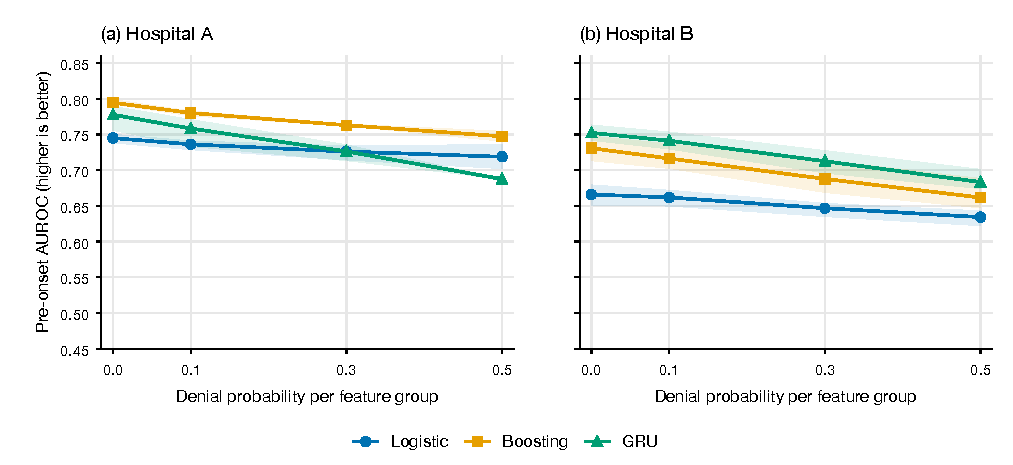
\includegraphics[width=\linewidth]{figs/paired_discrimination.pdf}
\caption{Pre-onset discrimination under increasing independent denial of laboratory and vital inputs. Points are means over three matched split seeds and shading spans their observed range, not a confidence interval. The vertical scale is restricted to emphasize differences in AUROC. Models are frozen and no consent-specific retraining occurs.}
\end{figure*}

\begin{figure*}[t]\centering
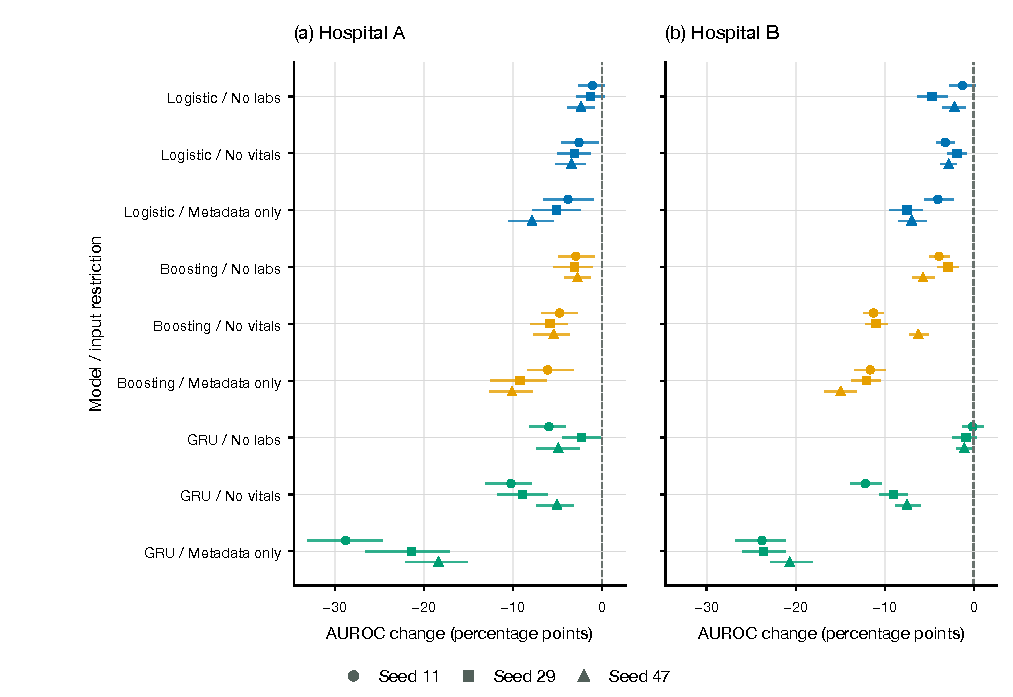
\includegraphics[width=\linewidth]{figs/paired_effects.pdf}
\caption{Paired AUROC differences for complete feature-group restrictions. Each point is one split seed and each interval is the pointwise 95\% percentile interval from 200 paired whole-patient bootstrap replicates. The same patient multiplicities are used in the full and restricted conditions. Intervals are not simultaneous across the displayed comparisons. Zero denotes unchanged AUROC, not an ethical or clinical acceptability threshold.}
\end{figure*}

\begin{figure*}[t]\centering
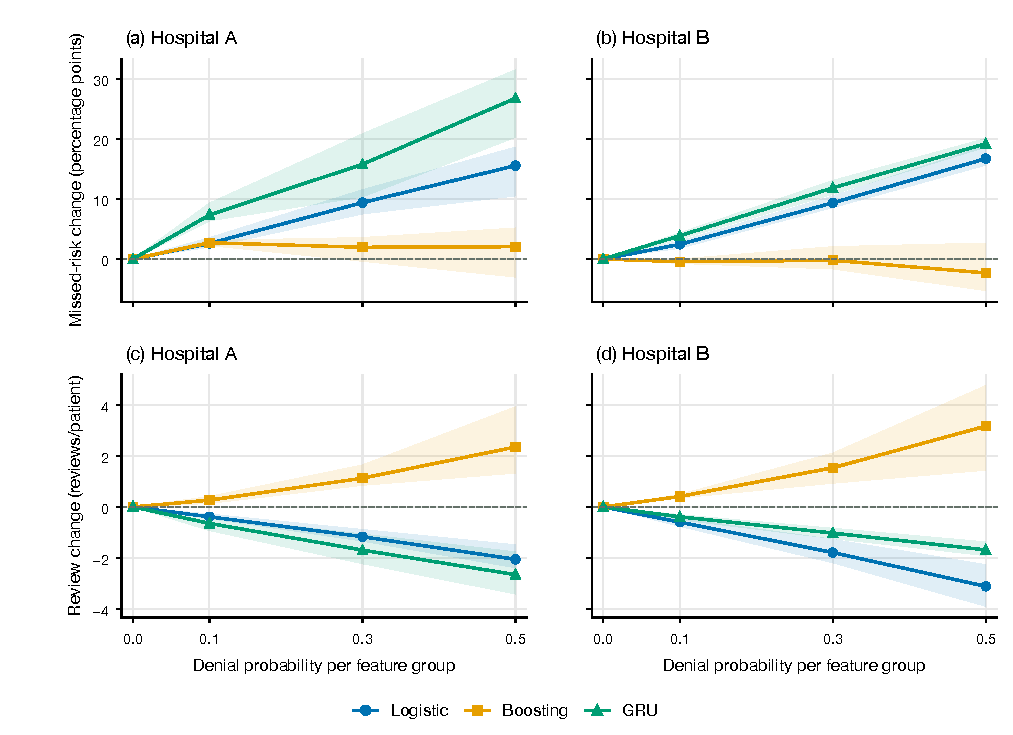
\includegraphics[width=\linewidth]{figs/paired_policy_effects.pdf}
\caption{Changes in missed-incident risk and review demand at fixed repeated-hourly alert thresholds. Positive risk change is deterioration; negative review change means fewer reviews. Lines are three-seed means and bands are descriptive seed ranges. All thresholds were selected on the original validation population and remain fixed across the denial-rate sweep. Paired policy confidence intervals are released separately.}
\end{figure*}

These comparisons answer a narrower, explicit version of the consent question: what happens to a frozen sepsis AI system when its permitted inputs change? They do not establish that the observed losses are unavoidable. Retraining under permitted features, adapting missingness handling or choosing a new validation-only threshold could change the outcome. Those are different interventions that would require separately evaluated models, rather than being folded into the same consent contrast. The present results also do not identify a clinically acceptable tolerance, so apparent similarity on an individual metric is not labeled non-inferiority.
